\documentclass{article}
\usepackage[final]{neurips_2019}
\usepackage{morris}

\usepackage{makecell}
\renewcommand\cellalign{tl}

% Some update to the NIPS template
\bibpunct{[}{]}{;}{n}{}{,}
\makeatletter
\renewcommand{\@noticestring}{Deep Learning, Sommer 2019, Universiteit van Amsterdam}
\makeatother

\renewcommand{\thesubsubsection}{\alph{subsubsection})}

\title{Assignment 2. Recurrent Neural Networks and Graph Neural Networks}
\author{%
  Maurice Frank\\
  11650656\\
  \href{mailto:maurice.frank@posteo.de}{maurice.frank@posteo.de} \\
  Code: \href{https://github.com/morris-frank/uvadlc_practicals_2019/tree/master/assignment_2}{github}
}

\begin{document}
\maketitle

\section{Vanilla RNN versus LSTM}
\subsection{RNN derivatives}
Generally we have:
\begin{align}
  \pf{\L}{\B{W}_{ph}}
  &= \pf{\L}{\B{p}} \pf{\B{p}}{\B{W}_{ph}}
\end{align}

With the two partials:
\begin{align}
  \pf{\L}{p_i}
  &= -\Σ_j y_j \pf{\log\hat{y}_j}{p_i}\\
  &= -\Σ_j \f{y_j}{\hat{y}_j}\pf{\hat{y}_j}{p_i}\\
  &= -y_i(1-\hat{y}_i) - \Σ_{j\neq i} \f{y_j}{\hat{y}_j} \· (-\hat{y}_i\hat{y}_j)\\
  &= -y_i + y_i\hat{y}_i + \hat{y}_i\Σ_{j\neq i} y_j\\
  &= \hat{y}_i \left(y_i + \Σ_{j\neq i} y_j\right) - y_i\\
  &= \hat{y}_i - y_i\\
  &\⇔\\
  \pf{\L}{\B{p}}
  &= \B{p} - \B{y}\\
\end{align}
Note here it holds \(\Σ_i y_i = 1\) because of the one-hot encoding.

The second derivative is more direct:
\begin{align}
  \pf{\B{p}}{\B{W}_{ph}}
  &= \B{h}^{(T)}\\
\end{align}

leads finally to:
\begin{align}
  \pf{\L}{\B{W}_{ph}}
  &= (\B{p} - \B{y}) \· \B{h}^{(T)}
\end{align}

The derivative with respect to the hidden weight we write down in its recursive form:
\begin{align}
  \pf{\L}{\B{W}_{hh}}
  &= \pf{\L}{\B{\hat{y}}} \pf{\B{\hat{y}}}{\B{p}} \pf{\B{p}}{\B{h}^{(T)}} \pf{\B{h}^{(T)}}{\B{W}_{hh}}\\
  \pf{\B{h}^{(T)}}{\B{W}_{hh}}
  &= \left(1 - {\B{h}^{(T)}}^2\right)\·\pf{}{\B{W}_{hh}}\B{W}_{hh}\B{h}^{(T-1)}\\
  &= \left(1 - {\B{h}^{(T)}}^2\right)\·\left[\left(\pf{}{\B{W}_{hh}}\B{W}_{hh}\right)\B{h}^{(T-1)} + \B{W}_{hh}\left(\pf{}{\B{W}_{hh}}\B{h}^{(T-1)}\right)\right]\\
  &= \left(1 - {\B{h}^{(T)}}^2\right)\·\left(\B{h}^{(T-1)} + \B{W}_{hh}\pf{\B{h}^{(T-1)}}{\B{W}_{hh}}\right)\\
\end{align}

Because we had to write down \(\pf{\L}{\B{W}_{hh}}\) recursively which we do not do for \(\pf{\L}{\B{W}_{ph}}\) we directly see the different length of the temporal dependencies in the two computational graphs.
For the hidden weights gradient we need to transverse the whole time-sequence while the other one only ever depends on the final hidden state.
This gives problems in practical training probable.
The partial gradients of the hidden weights might be small and they form a product.
The gradient might be vanishing.
In practice this might go so far to reach the numerical limits of floating point arithmetics.

\subsection{Vanilla RNN code}
Find the code inside \texttt{vanilla\_rnn.py} and \texttt{train.py}.

\subsection{Vanilla RNN experiment}
See Figure~\ref{fig:accuracy_loss} for a overview plot of the results and Section~\ref{sub:lstm_practice} for a discussion/comparison of the results.

\subsection{Optimizer}
SGD has problems.
One of them is occurring oscillations in valleys of the loss space.
SGD does not have any \textit{memory} and thus just tries to approximate the currents face's gradient to follow down which might make the path jump around a minimum of the valley.
One change to counter this problem is introducing \textbf{momentum}.
Following the intuition of the physical term, the gradient with momentum gets only changed gradually not sudden in every optimizer step.
This is implemented as a decaying average of gradient updates.
The weights get updated as a weighted sum of the previous update and the new gradient.
A second idea is to tweak the learning rate for each weight and not use a fixed \(\eta\) for all, yielding a \textbf{adaptive learning rate}.
For those weights that change a lot (bounce around some valley) we want to reduce the update step to counteract the bouncing.
This can be seen in the RMSProp~\citep{hinton2014} optimizer as described below:
\begin{align}
  v_t &= \rho v_{t-1} + (1-\rho) \· {(\nabla_{\θ_t}f)}^2\\
  \θ_{t+1} &= \θ_t - \f{\eta}{\sqrt{v_t + \ε}} \· \nabla_{\θ_t}f
\end{align}
\(\rho\) defines the decaying sum. We compute the update but than divide the learning rate \(\eta\) for each weight by the new update.
Thus oscillating weights will get a smaller update.
Adam~\citep{kingma2014} optimizer works quite similar:
\begin{align}
  v_t &= \β_1 \· v_{t-1} - (1 - \β_1) \· \nabla_{\θ_t}f\\
  s_t &= \β_2 \· s_{t-1} - (1 - \β_2) \· {(\nabla_{\θ_t}f)}^2\\
  \θ_{t+1} &= \θ_t - \f{\eta}{\sqrt{s_t + \ε}} \· v_t
\end{align}
We also adapt the learning rate per weight by dividing by the square-root of the  squared gradients.
But here also directly use the momentum but having the decaying sum of weight-wise gradients. \(\β_1 \text{and} \β_2\) are tuneable hyperparameters.

\subsection{LSTM theory}
\subsubsection{LSTM Gates}
\begin{description}
  \item[\I{input modulation gate} \(\B{g}^{(t)}\)] The input modulation gate determines candidate information from the new input (using also the old hidden state).
  We want our state values normalized but need also negative values (otherwise the cell values would only increase) which, as in this case, can be done with a \(\tanh \), squashing the input to \([-1, 1]\).
  \item[\I{input gate} \(\B{i}^{(t)}\)] The input regulates which and how much information of the input of this time step should be included in the cell and hidden state.
  As the input gate regulates the flow it is necessary to have its values bounded to \([0,1]\) which can most directly achieved by squashing the values with the sigmoid.
  \item[\I{forget gate} \(\B{f}^{(t)}\)] The forget gate regulates which and how much information from the old cell state should be disregarded under the new information from the input (and the old hidden state).
  As the forget gate only changes the importance (magnitude) of the information in the cell state it should be in \([0,1]\) which is achieved with the sigmoid.
  \item[\I{output gate} \(\B{o}^{(t)}\)] The output gate regulates which and how much information from the new cell state should go into the new hidden state.
  Again its gating the values from the other tensor which is asking for a range \([0, 1]\) achieved by the sigmoid.
\end{description}

\subsubsection{Number of parameters}
We have given \(\B{x}\∈\ℝ^{T\×d}\) with \(T\) sequence length and \(d\) feature dimension.
Further we have \(n\) hidden units.
Then we have
\begin{equation*}
  4\· (d\·n + n\·n + n)
\end{equation*}
trainable parameters for \textit{one} LSTM cell.
If we want to include the projection onto the classes \(c\) the size increases of course to:
\begin{equation*}
  4\· (d\·n + n\·n + n) + n\·c + c
\end{equation*}

\subsection{LSTM practice}\label{sub:lstm_practice}
Find the code inside \texttt{lstm.py} and \texttt{train.py}.

We train the two models (RNN and LSTM) for palindromes with sizes 5 up to 40.
Both models get a hidden size of 128.
As optimizer we use  RMSprop with a learning rate of \(0.001\) until convergence of the loss.
The weights for both models are initialized with He initialization~\cite{he2015} as it performs well compared to plain normal init.

For a overview of the results check out Figure~\ref{fig:accuracy_loss}.
We see in general that the LSTM is able to learn the palindromes faster and for longer sequences.
The RNN is only able to improve on randomness (\(=\) accuracy of 0.1) up to length 17.
Further the RNN is only able to reach full accuracy for palindromes smaller than 10.
The LSTM reaches perfect accuracy for all lengths but we see that for length of 23 we do not see improvement over randomness until almost 3000.
If run for long enough the LSTM learns full accuracy for all tested lengths but we found that not be the interesting result here.
The LSTM learning slower at higher lengths is explained in that we use the same hyperparameters for all experiments especially the learning rate.
An optimization of the hyperparameters for the LSTM might speed up training for longer sequences.
The experiment clearly shows that the LSTM is more capable of learning longer dependencies.

\begin{figure}
  \centering
  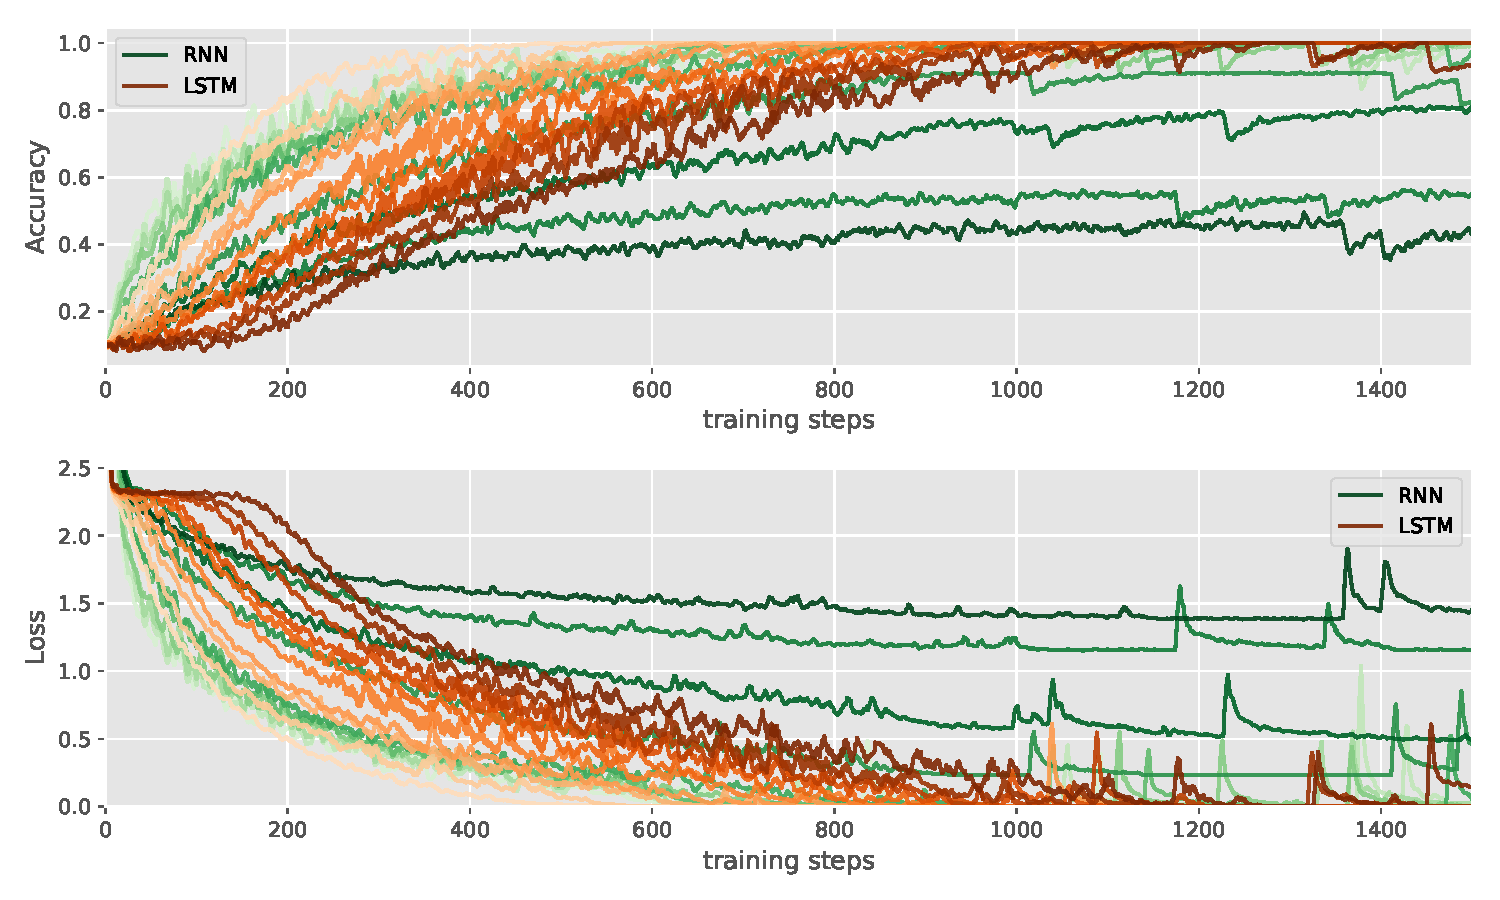
\includegraphics[width=\linewidth]{assignment_2/part1/palindrome.pdf}
  \caption{\B{Top} the accuracy and \B{bottom} the loss while training.
  Lightness of the color codes the palindrome length ranging from 5 numbers at the lightest color in steps of 2 to 23 numbers at the darkest color.
  (making 9 curves per model). All curves are an average of ten runs and smoothed with a box filter with width 10 for better readability. Note that two of the RNN curves never increase over 0.1 in the accuracy plot.}\label{fig:accuracy_loss}
\end{figure}

\section{Recurrent Nets as Generative Model}
\subsection{Learning English from South Park and the Moses}
In these experiment we train a simple character-level language model with LSTM.
We train from texts from the bible and the television show South Park.

\subsubsection{The Implementation}
Find the code inside \texttt{model.py} and \texttt{train.py}.

We implement the basic character-level language model using two stacked LSTM cells (three for the second experiment).
Both cells are followed by a Dropout unit.
We use a linear projection to project the hidden state from the second LSTM down on the class predictions.
As we get a sequence of characters as input we use an embedding with fixed identity weights (one-hot encoding) to process the input for the LSTM.
We set the hidden size of both cells to 128.
The dropout layer is set at 0.05 dropout probability.

We train the model with the Adam optimizer feeding it sequences of 30 characters from the text in mini-batches of 64.
The initial learning rate is set at 2e-3.
Further we decay the global learning rate every 5000 steps by 0.04.

We preprocess the text files by reducing the set of characters.
All text is made lowercase and line breaks are removed.
We remove special, uncommon characters (e.g. acutes from German and Spanish) replacing them: e.g. ö \(\to\) o and\ ;\ \(\to\)\ ,.

\subsubsection{The results}
For training we feed the model with all transcripts of the television series \textbf{South Park}.
In total the transcript have 813k words.
See Figure~\ref{fig:training_southpark} for the training progress in the first 1e5 steps.

To understand the generative power of our model qualitatively we sample from the language model at different steps during training.
Sampling is done by picking a first character uniformly by random.
Next we iteratively feed the character into the model generate new hidden and cell states.
From the hidden state we can sample a new character under different temperatures.
The new character is saved in the string and fed back to the model with the new hidden and cell state.
We do this until we reached the desired output length.

Following are text samples of length 20, 30, 50 and 120 at step 0, 1e4, 2e4, 3e4, 4e4, 5e4, 1e6, 2e6 and 5e6.
Each step we sample at temperatures \(T\in\) 0, 0.5, 1 and 2.0.
Note that temperatures 0 corresponds to greedy sampling, meaning we pick the character with the highest probability.

\vspace{1em}

\hspace*{-0.2\textwidth}\resizebox{1.4\textwidth}{!}{
\begin{minipage}{0.7\textwidth}
\begin{tabularx}{\textwidth}{ccX}
\multicolumn{3}{c}{\Large {0}}\\\toprule
Temp & l & Samples \\ \toprule
\multirow{4}{*}{0.0}
& 20 & \makecell{riiiiiiiiiiiiiiiiiii}\\& 30 & \makecell{5iiiiiiiiiiiiiiiiiiiiiiiiiiiii}\\& 50 & \makecell{ iiiiiiiiiiiiiiiiiiiiiiiiiiiiiiiiiiiiiii\\iiiiiiiiii}\\& 120 & \makecell{oiiiiiiiiiiiiiiiiiiiiiiiiiiiiiiiiiiiiiii\\iiiiiiiiiiiiiiiiiiiiiiiiiiiiiiiiiiiiiiii\\iiiiiiiiiiiiiiiiiiiiiiiiiiiiiiiiiiiiiiii}\\\midrule
\multirow{4}{*}{0.5}
& 20 & \makecell{yjw2b3b6	­d.	w,m54tw}\\& 30 & \makecell{7-edbx2)dg4­7syam  enlahv  sx-}\\& 50 & \makecell{r8'/du1c6qzc1si7.lklsmwoui"xzn 68-a8gg z\\w"e))!/pb6}\\& 120 & \makecell{kee,e),j8noza,a/6e­ra""h	'f'a79d'0g u'ya\\!­r-(opt,s(t	ode)!,,hz3z9(sc'jq/b zpr5 c\\txlm9uid(bnd9zr6/,p	 1­peg!m	­zxh	?7nskx}\\\midrule
\multirow{4}{*}{1.0}
& 20 & \makecell{e!28jn25(1815yzwthr3}\\& 30 & \makecell{0..fg'(iaa 9' x )d6a	81i7oabaf}\\& 50 & \makecell{ptnctn­,h	k.-6ybi1b1/,mdf5a(8xenxmmu7bsx\\du3lvt95b9}\\& 120 & \makecell{rx54 ?5taif"cs1c)!a36wsy0'2eodj6/?y.5yq?\\q/2 ocy5,(ctzq'1n?sojh38 hgp() 9m3.p9lhs\\7918h3l 1 f1"0.­3s13ve	zk' ,-u85(tt dp}\\\midrule
\multirow{4}{*}{2.0}
& 20 & \makecell{ar8ld7gb7n!s5pzxj	5f}\\& 30 & \makecell{uf­ur),f­c2o)h9hy?r9.fkp­8)8wv}\\& 50 & \makecell{jkw(-unz1vm'n3" /?r6rz(le0  c8q k0(	p­ff\\4.oy7)sa­3}\\& 120 & \makecell{?-pi!'8l6)n-qj/50,j.­aq7!ebjvnm! "c02mj \\,0t9	vekhj-7zbw-8f6j-dzq?-m,(q7z"73s)7-u\\rn	eqt "­d2omjji8 (7j30xylc9ore.ubon762i}\\\midrule
\end{tabularx}
\end{minipage}
\begin{minipage}{0.7\textwidth}
\begin{tabularx}{\textwidth}{ccX}
\multicolumn{3}{c}{\Large {10000}}\\\toprule
Temp & l & Samples \\ \toprule
\multirow{4}{*}{0.0}
& 20 & \makecell{me to the stupid stu}\\& 30 & \makecell{re to the strange of the stupi}\\& 50 & \makecell{ that's not the power to the boys are go\\nna be a}\\& 120 & \makecell{ze is the problem than the problem to th\\e popped to the balls are gonna be so th\\e problem that the problem of the part o}\\\midrule
\multirow{4}{*}{0.5}
& 20 & \makecell{! i know i thought i}\\& 30 & \makecell{11 and sooo and then we can be}\\& 50 & \makecell{got a spilitory. the hell are you beauti\\ful his mo}\\& 120 & \makecell{/fuck your son in your new problem and i\\'m sure your looks like the lately his n\\ight to the bame! and we have to play wi}\\\midrule
\multirow{4}{*}{1.0}
& 20 & \makecell{­rish are dellagin's}\\& 30 & \makecell{hiltor. alto si- .  disolant s}\\& 50 & \makecell{quacking are on mandayout kike the burg.\\ that's? k}\\& 120 & \makecell{lor place! all what we've reading much-b\\leh"is is brolly hangh! keep you! i'm ju\\st gonna kill by a hot. .r. tom. yeah! h}\\\midrule
\multirow{4}{*}{2.0}
& 20 & \makecell{yed. yoh,! whaa, wha}\\& 30 & \makecell{, huh8mu, nsy! oh what,!,'yeaw}\\& 50 & \makecell{ yetriuze be bocy toks. ugs!.4" - you ju\\st lose wi}\\& 120 & \makecell{(122.  peofjies, bervltsalyfatquemasine,\\ you'do've fwire 69fven cull,! bye.!!)!.\\me! it's  ville,""days, sv.!.l poft one }\\\midrule
\end{tabularx}
\end{minipage}
\begin{minipage}{0.7\textwidth}
\begin{tabularx}{\textwidth}{ccX}
\multicolumn{3}{c}{\Large {20000}}\\\toprule
Temp & l & Samples \\ \toprule
\multirow{4}{*}{0.0}
& 20 & \makecell{9 the stupid people }\\& 30 & \makecell{ and the stupid asshole!  wh}\\& 50 & \makecell{g and the principal problem with the stu\\dents and }\\& 120 & \makecell{can that the students and the students a\\nd the police and the police and started\\ to the police and state the part of the}\\\midrule
\multirow{4}{*}{0.5}
& 20 & \makecell{-hold on.  god damni}\\& 30 & \makecell{)  that's what i don't have a }\\& 50 & \makecell{ou want to show the poor more than your \\problem st}\\& 120 & \makecell{5 from here for here!  we can do it for \\a boy is for a bad of the planet. what a\\re we gonna do it out! what are we gonna}\\\midrule
\multirow{4}{*}{1.0}
& 20 & \makecell{tle son is so any ne}\\& 30 & \makecell{quut up and shows! we want it?}\\& 50 & \makecell{fell is whatever if here in the stuff th\\at we coul}\\& 120 & \makecell{! grabba basky with a news. no, kyle. ma\\ybe you talk to you that? i don't know y\\our veal. my pockets, zammate your legra}\\\midrule
\multirow{4}{*}{2.0}
& 20 & \makecell{8 totarnap quiete ch}\\& 30 & \makecell{(clein! lond.,ncomaa-lopeous c}\\& 50 & \makecell{p.,"" nice, nobody! g'ee!! yemph.) o-how\\seefo elea}\\& 120 & \makecell{2!...lu-yuwwakkih? caugh. ""n'tcufort, d\\nivo wegghy newra! geraldon(ensides you \\know! in-carv twa! (dudd-k egerpizpsnc. }\\\midrule
\end{tabularx}
\end{minipage}
}
\par
\hspace*{-0.2\textwidth}\resizebox{1.4\textwidth}{!}{
\begin{minipage}{0.7\textwidth}
\begin{tabularx}{\textwidth}{ccX}
\multicolumn{3}{c}{\Large {30000}}\\\toprule
Temp & l & Samples \\ \toprule
\multirow{4}{*}{0.0}
& 20 & \makecell{per the problems and}\\& 30 & \makecell{e the problem is a little boys}\\& 50 & \makecell{n the protect the probably in the contro\\l of the p}\\& 120 & \makecell{-  and i don't know what i was the paren\\ts are the stuff and i was the problem t\\han the park country in the state to the}\\\midrule
\multirow{4}{*}{0.5}
& 20 & \makecell{?  oh my god!  well,}\\& 30 & \makecell{g all the kids hate your vampi}\\& 50 & \makecell{/friends to put the bus. well, sure is a\\ little fu}\\& 120 & \makecell{day cartman! it sure is true. he's kille\\d, and i want to do is what you understa\\nd that there was my friends and some ho}\\\midrule
\multirow{4}{*}{1.0}
& 20 & \makecell{me act now. that's w}\\& 30 & \makecell{give me, even going up with my}\\& 50 & \makecell{2s? i don't know a people have a lot of \\words agai}\\& 120 & \makecell{5 down't you guys are not all the show t\\ogety goddamned doctor is a crow, butter\\s! that does with ana good oraig, where'}\\\midrule
\multirow{4}{*}{2.0}
& 20 & \makecell{n aypofa? yeah!!) u }\\& 30 & \makecell{quedsplove., not theared lovin}\\& 50 & \makecell{yw. xlezs, v mrto! govertuh you ya! um r\\test. hyeh}\\& 120 & \makecell{6e-c6? ma'poghutlike,"waitbmecy. a adulc\\cuma"' zey ninety, 3.6 wqi-fs' woman?! k\\yre? thh). wamnasniqnl 4) i-cake it gly }\\\midrule
\end{tabularx}
\end{minipage}
\begin{minipage}{0.7\textwidth}
\begin{tabularx}{\textwidth}{ccX}
\multicolumn{3}{c}{\Large {40000}}\\\toprule
Temp & l & Samples \\ \toprule
\multirow{4}{*}{0.0}
& 20 & \makecell{ the stupid ass of t}\\& 30 & \makecell{the stuff in the students and }\\& 50 & \makecell{you guys are gonna be a children and sta\\y out of h}\\& 120 & \makecell{s and the problem that the state of the \\students and the problem that the studen\\ts and start a second of the stupid ass }\\\midrule
\multirow{4}{*}{0.5}
& 20 & \makecell{ll you have a drink }\\& 30 & \makecell{t that that we got reality who}\\& 50 & \makecell{t his son's friends and a second. you gu\\ys take a }\\& 120 & \makecell{call my house. that thing is stoppin' he\\r canadian for a time!  ...and i know ho\\w you wanna do this and well then i have}\\\midrule
\multirow{4}{*}{1.0}
& 20 & \makecell{ dreambit careful, i}\\& 30 & \makecell{xice how me a mall eating. tha}\\& 50 & \makecell{ball maybe insurted on our odmedent. it'\\s not on t}\\& 120 & \makecell{aking a bunch about you! alright.  oh, c\\ows! that's nice back that does. and uh \\yeah, it'll get the titzolisy.  six stor}\\\midrule
\multirow{4}{*}{2.0}
& 20 & \makecell{-e! your habsy. eric}\\& 30 & \makecell{7395.""-" stapa.nlona ded, you}\\& 50 & \makecell{iand quest monmils, eric. moutupt a!!! t\\hanks, cla}\\& 120 & \makecell{ah'-! ...ohrs, who duid "c? calmndy!) ta\\?! uh tox into ys-ave. shho! o-kay! you,\\ 9, quickly. (kittle koek!!r me cy were }\\\midrule
\end{tabularx}
\end{minipage}
\begin{minipage}{0.7\textwidth}
\begin{tabularx}{\textwidth}{ccX}
\multicolumn{3}{c}{\Large {50000}}\\\toprule
Temp & l & Samples \\ \toprule
\multirow{4}{*}{0.0}
& 20 & \makecell{-  and then i can se}\\& 30 & \makecell{f the students are so that the}\\& 50 & \makecell{ing to see you all the start on the part\\y of the p}\\& 120 & \makecell{re a little boy in the principal stupid \\asshole!  what the hell are you doing? i\\ don't know what i can do it all the stu}\\\midrule
\multirow{4}{*}{0.5}
& 20 & \makecell{good, the only perso}\\& 30 & \makecell{10 people who present. you don}\\& 50 & \makecell{2 mm. cartman, you're not going to make \\them bette}\\& 120 & \makecell{s on the people be a little boy the stat\\us of her there. tell you in here. i can\\'t take it anymore was some construction}\\\midrule
\multirow{4}{*}{1.0}
& 20 & \makecell{okay. 'cause you com}\\& 30 & \makecell{ll i've... good way, and sweet}\\& 50 & \makecell{7 friends off, too. my legs of force her\\e he give }\\& 120 & \makecell{	pash! you decighcion the poxauld first \\comes in trualing that saying this time.\\ oh yeah. okay kids, donleya! ned genefi}\\\midrule
\multirow{4}{*}{2.0}
& 20 & \makecell{u don't know.  riva }\\& 30 & \makecell{julth not an/mh??pkmman! holy,}\\& 50 & \makecell{tyal! we!sex, subbeld's bad alright-.,i \\mul!  bemp}\\& 120 & \makecell{?,'-  uh i camebokalo's?!!iravy?!  oh, s\\top!-uw, all, uuuf-if there suddes8 her?\\ unfniyor mado. start! afriewt.!  your l}\\\midrule
\end{tabularx}
\end{minipage}
}
\par
\hspace*{-0.2\textwidth}\resizebox{1.4\textwidth}{!}{
\begin{minipage}{0.7\textwidth}
\begin{tabularx}{\textwidth}{ccX}
\multicolumn{3}{c}{\Large {100000}}\\\toprule
Temp & l & Samples \\ \toprule
\multirow{4}{*}{0.0}
& 20 & \makecell{f the stupid asshole}\\& 30 & \makecell{we have to get the star really}\\& 50 & \makecell{u guys are the only thing to do it there\\ and i don}\\& 120 & \makecell{80 per cent to the soul of the state and\\ so the school stay away from the countr\\y is a big deal with the start a second }\\\midrule
\multirow{4}{*}{0.5}
& 20 & \makecell{ke the pain! we want}\\& 30 & \makecell{2000, i'm a big and i can't do}\\& 50 & \makecell{ou guys! yeah, we have to work at my bod\\y. i don't}\\& 120 & \makecell{we have to kill you six hours. they did \\it!  the things to get a really seeing t\\he one things is. we are the brains and }\\\midrule
\multirow{4}{*}{1.0}
& 20 & \makecell{ht at us saw... all }\\& 30 & \makecell{? don't they come a meters! wh}\\& 50 & \makecell{, you know what they aren't any of that \\guy travel}\\& 120 & \makecell{? really?  you have to be costaiint. so,\\ nuh dougless is the confederated chinpo\\kes you dope? could you land it... sandw}\\\midrule
\multirow{4}{*}{2.0}
& 20 & \makecell{, ver disk thos girl}\\& 30 & \makecell{(k. graswmak!! hs, ly- wen'- n}\\& 50 & \makecell{4 ! eric cat, kyloh, ,-mosely!'-'sssuper\\ing.s waal}\\& 120 & \makecell{? bopha nicpdorations, a chinaple th you\\r -rect kickin'cybun tripi and 'cd"of-)-\\whh ibz. yem.y?) oh... with?. (hm.!)  if}\\\midrule
\end{tabularx}
\end{minipage}
\begin{minipage}{0.7\textwidth}
\begin{tabularx}{\textwidth}{ccX}
\multicolumn{3}{c}{\Large {200000}}\\\toprule
Temp & l & Samples \\ \toprule
\multirow{4}{*}{0.0}
& 20 & \makecell{xt to the bathroom a}\\& 30 & \makecell{40000 per cent of the state of}\\& 50 & \makecell{(a friend is a little bit of a bitch!  w\\hat the he}\\& 120 & \makecell{n the stupid party of the store for the \\second that the world is a little boy wh\\o was the problem.  what are you doing? }\\\midrule
\multirow{4}{*}{0.5}
& 20 & \makecell{85 dollars signing t}\\& 30 & \makecell{ing the town of a super be sat}\\& 50 & \makecell{00 per cent of them. hello eric, that's \\it there. }\\& 120 & \makecell{ke in a son is about to be a big deal to\\ god is having a new town of all the red\\ life in sandwich thing? so for you to s}\\\midrule
\multirow{4}{*}{1.0}
& 20 & \makecell{for that idea.  are }\\& 30 & \makecell{) doh, if a scott. i know  we'}\\& 50 & \makecell{) your sriss of mouths of charge of you \\de by him }\\& 120 & \makecell{r you now bitching my part of my towelie\\!! i know it here? look, we will cut off\\ my balls, red measure?! get your grandm}\\\midrule
\multirow{4}{*}{2.0}
& 20 & \makecell{goaj.  (go we'll bo,}\\& 30 & \makecell{evweac eated itge-joren l.? i }\\& 50 & \makecell{'ve gravi my vacco.,''s?? kewnu , ms. ng\\-ctdai.,mi}\\& 120 & \makecell{872!0 yuk. ?que? whe- hey mirgith rouetn\\put yoba goddami-enga!"" go back with 3/\\5. obceaob, ike, 'f's lots autlakffful i}\\\midrule
\end{tabularx}
\end{minipage}
\begin{minipage}{0.7\textwidth}
\begin{tabularx}{\textwidth}{ccX}
\multicolumn{3}{c}{\Large {500000}}\\\toprule
Temp & l & Samples \\ \toprule
\multirow{4}{*}{0.0}
& 20 & \makecell{x and then i can see}\\& 30 & \makecell{, i want to be a company that }\\& 50 & \makecell{quite a lot of money to see the start a \\lot of mor}\\& 120 & \makecell{5 month.  what are you doing? we have to\\ do it the students are the one that the\\ world is a little bit of the problem.  }\\\midrule
\multirow{4}{*}{0.5}
& 20 & \makecell{­  i don't feel so m}\\& 30 & \makecell{3 dollars. i love you guys, i }\\& 50 & \makecell{/11 has pretty good to go one different \\boys and f}\\& 120 & \makecell{2002! he was the united states with the \\armas place in the fish and that's okay.\\ all right, we are so funny! we can do i}\\\midrule
\multirow{4}{*}{1.0}
& 20 & \makecell{w, that noticed you!}\\& 30 & \makecell{- she's too...  ruuuurribuy! t}\\& 50 & \makecell{10,000 one to this out of hero...you'll \\meet a daw}\\& 120 & \makecell{gonna build your flute boy in my olved q\\uit. go sure. it's serious! every piss, \\huh?! oh,  hey, changedage the stupid au}\\\midrule
\multirow{4}{*}{2.0}
& 20 & \makecell{).qh avoid theng  "h}\\& 30 & \makecell{- ad zumir's reevc dlamlant! l}\\& 50 & \makecell{ub! yeephclexto, cartman, the run. o,,..\\) boy. ste}\\& 120 & \makecell{-  get mm."" nribly  dude! p-juros.!lfiz\\e i bb gallawes---c-curity!"" caren soga\\rth! right ninleyts, garyeow? i'm i?"...}\\\midrule
\end{tabularx}
\end{minipage}
}
\vspace{1em}

We see some general trends.
At temperature of 2.0 the model never able to form words which suggests that this is too high.
Most interesting we see the model being able to generate almost coherent sentence early on in training as e.g.\ at step 1000 with \(T=0.5\).

In a second experiment we feed the network the \textbf{five books of Moses} from the old testament.
Compared to the previous transcript this text only has 156k words.
We extend the model architecture to check if that increases the generative power.
For that we us \textit{three} stacked LSTM cells.
Further we feed sequences of 40 characters and decay the global learning rate only all 20k steps.
All other parameters are set as before.

Trainings progress was similar to the first experiment so we just give exemplary qualitative results below.

\begin{figure}
  \centering
  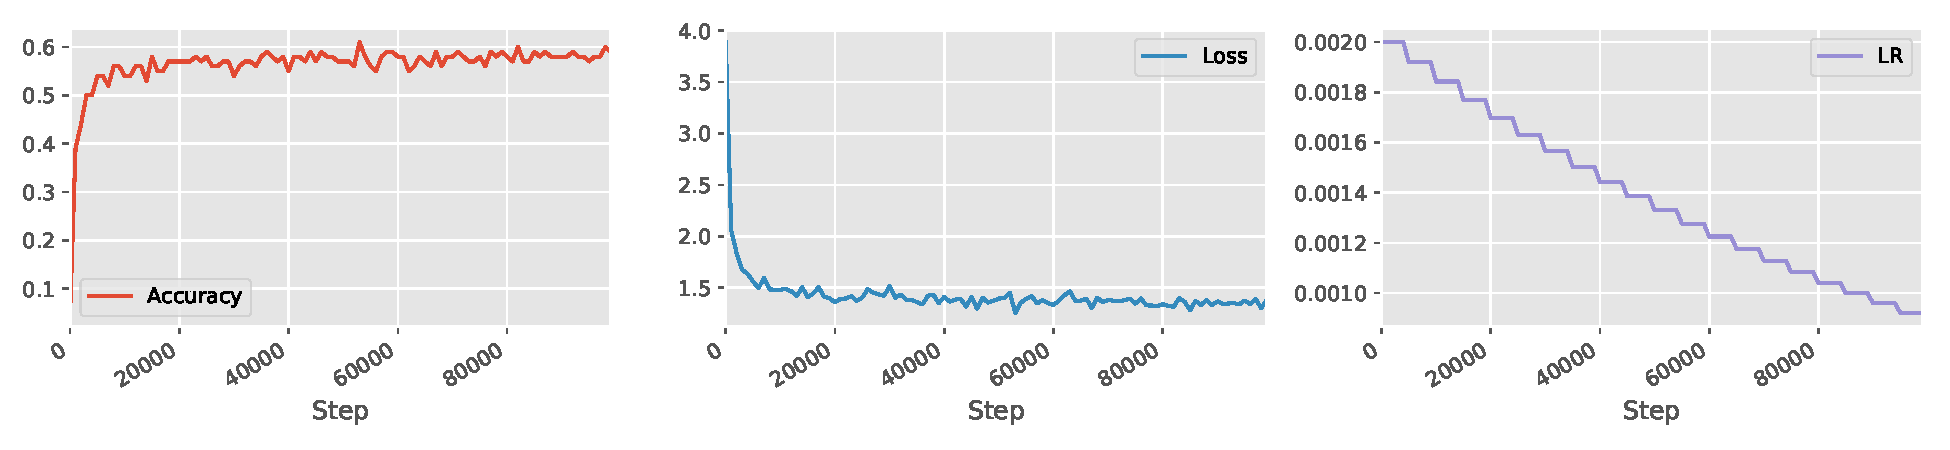
\includegraphics[width=\linewidth]{assignment_2/part2/results/southpark_2/southpark.pdf}
  \caption{Accuracy, Loss and the decaying Learning Rate for the LSTM language model during training using the South Path transcripts.
  Note that accuracy and loss are a bad surrogate for our task as they describe the capability of the model to predict the next character given a string while our actual goal is to get a generative model.}
  \label{fig:training_southpark}
\end{figure}

\section{Graph Neural Networks}
\subsection{Forward Layer}
\subsubsection{Message passing in a GNN}
The \(\hat{A}\) matrix contains the edge information between the nodes in the graph.
This includes the self-connections of all nodes from the identity \(\1_N\).
We update the activations with \(H^{l+1} = \σ(\hat{A}H^{(l)}W^{(l)})\).
So we update the activation associated with one node only for the activations of edges that have non-zero edge weights in \(\hat{A}\).
A node is changed by the nodes its connected to.
In reverse we can see that information in one node can propagate to all connected adjacent nodes in one time step which can be visualized as the message passing over the graph.

\subsubsection{How many layers to propagate a message along three hops?}
In every layer of the GCN you can propagate information along one edge so to let information reach a node three hops away we would need three layers.

\subsection{Applications of GNN}\label{sub:applications_gnn}
In \textit{Multi-Granularity Reasoning for Social Relation Recognition from Images}~\cite{zhang2019} the authors build graphs on images of humans.
The graphs describe first the relationship of a person in the image with its surrounding objects amongst other things other persons in the image.
A second graph represents the pose of each person in the image.
On these two types of graphs they use Graph Convolutional Networks (GCN) to predict the social relationship of these persons.
For example in an image of parent and child the bending pose of the parent and the connection of the two persons in the Person-Object graph lets the method infer their relationship.

Next in \textit{Disease Prediction using Graph Convolutional Networks: Application to Autism Spectrum Disorder and Alzheimer's Disease}~\cite{parisot2018} propose to use GCN for medical image processing.
The nodes of the graph in this setting are features of medical image acquisitions which in their experiments are gathered from structural and functional MRI.
As they predict the health state of multiple individuals at once the graph consists of many image features of multiple persons.
The edges here describe the phenotypical similarity between two individuals which are described by categorical medical data (e.g.\ sex).
The GCN uses this graph to predict the health state of the population.


Lastly in \textit{Temporal Relational Ranking for Stock Prediction}~\cite{feng2019} we seen an application of GCN in stock prediction.
Here the nodes are features capturing the historical information of one stock and the edges capture the relations between two companies stock.
Both historical intra and inter stock features are generated by LSTM from historical stock data.
Again we build a graph from the edges and nodes and use GCN to predict in this case the stocks next day performance at the market.

\subsection{Comparison and Combination of GNN and RNN}
\subsubsection{Comparing GNN and RNN}
Using a RNN assumes our data is orderable along one axis, meaning every node of information is at most connected to one \textit{previous} and one \textit{next} node of information and that no two nodes have the same previous or next node.
For the GNN we assume data whose node of information is related to an irregular number of other nodes.

One major difference for the two is that the GNN can give edges between, relationship between to states, a weight or a feature itself.
For the RNN we assume a equidistant (temporal etc.) edge between each node while for the graph we can adjust this.


\subsubsection{Combining GNN and RNN}
We saw such a combination of RNN and GNN models in Section~\ref{sub:applications_gnn} already. The work on prediction of stock markets used LSTM and GCN in conjunction.
In there each node of graph related to a linear temporal structure, the historic sock data.
As those linear temporal graphs where themselves related to each other one can use a graph model to analyze.

The reverse idea also seems plausible by using a RNN to go over nodes of graphs.
Imaginable might here be an application where the data is organized in a graph, let's say a social graph, but is subject to temporal changes.
A GNN could be used to analyze the state of the graph at one given point while the RNN uses these temporal states and can for example predict future states from that.

\bibliographystyle{unsrtnat}
\bibliography{references}

\end{document}
